The physics program of CMS has achieved incredible results in its first 2 runs including the discovery of the Higgs boson.
The Higgs discovery completes the standard model (SM) of particle physics.  
Despite this incredible achievement, many mysteries beyond the (SM) remain including understanding the hierarchy problem,
the nature of dark matter, and the origin of the matter-antimatter asymmetry in the universe.  

Therefore, the CMS program continues to study the SM in great detail and probe for signs of beyond the SM physics.  
For the continued success of CMS physics program, CMS plans accumulate an unprecedented amount of data, approximately $3~ab^\text{-1}$, to be delivered by the (high luminosity) HL-LHC.  
This dataset will be approximately 100 times larger than our current LHC dataset.  
Although we will accumulate an unprecendented dataset, we will have to deal with increasingly complex enviroments characterized by
extreme levels of pileup.  
Pileup is defined as p-p interactions, produced in addition to the interaction of interest.
They serve to add noise to the detection of particular physics processes and degrade the performance and sensitivity of CMS.
During the HL-LHC runs, there are expected to be approximately 140-200 pileup interactions per proton bunch crossing. 
So while we will have an unprecedented amount of data, we will need to maintain the current physics performance of the CMS detector in order to maximize the HL-LHC run.

In particular, one primary issue related to the additional pileup is the increased trigger rates.  
The purpose of CMS trigger system is to determine and save the most interesting physics events.
Without an efficient trigger system we would not save the right events to permanent storage and would thus lose important physics. 
The collision rate at the (HL-)LHC is 40~MHz.  
The trigger system, during the HL-LHC, will be required to reduce that rate to a more manageable rate of $\sim5~$KHz~\cite{Contardo:2020886}.  
This data reduction occurs through a 2-layer system: in level-1 (L1), hardware and fast electronics are used to reduce the rate to approximately 700~KHz; and in the second layer, the high level trigger (HLT), the rate is reduced down to approxiately 5~KHz.  
We focus in this document on the design and implementation of a L1 hardware trigger.  
External constraints and the size of detector buffers constrain the time of the L1 decision to be approximately $12.5~\mu s$.  
The L1 trigger system includes information from the calorimeters and muon systems, and new for the HL-LHC, it will also include tracker information.  
The system is illustrated in Fig.~\ref{fig:overview}.
In this document we focus on the design and performance of the "correlator" system, denoted in Fig.~\ref{fig:overview}.
With the new tracking information avaialable in the L1 trigger for the HL-LHC, the L1 trigger algorithms can be completely 
redesigned and the perforamnce can be greatly improved.

\begin{figure}[htb]
\centering
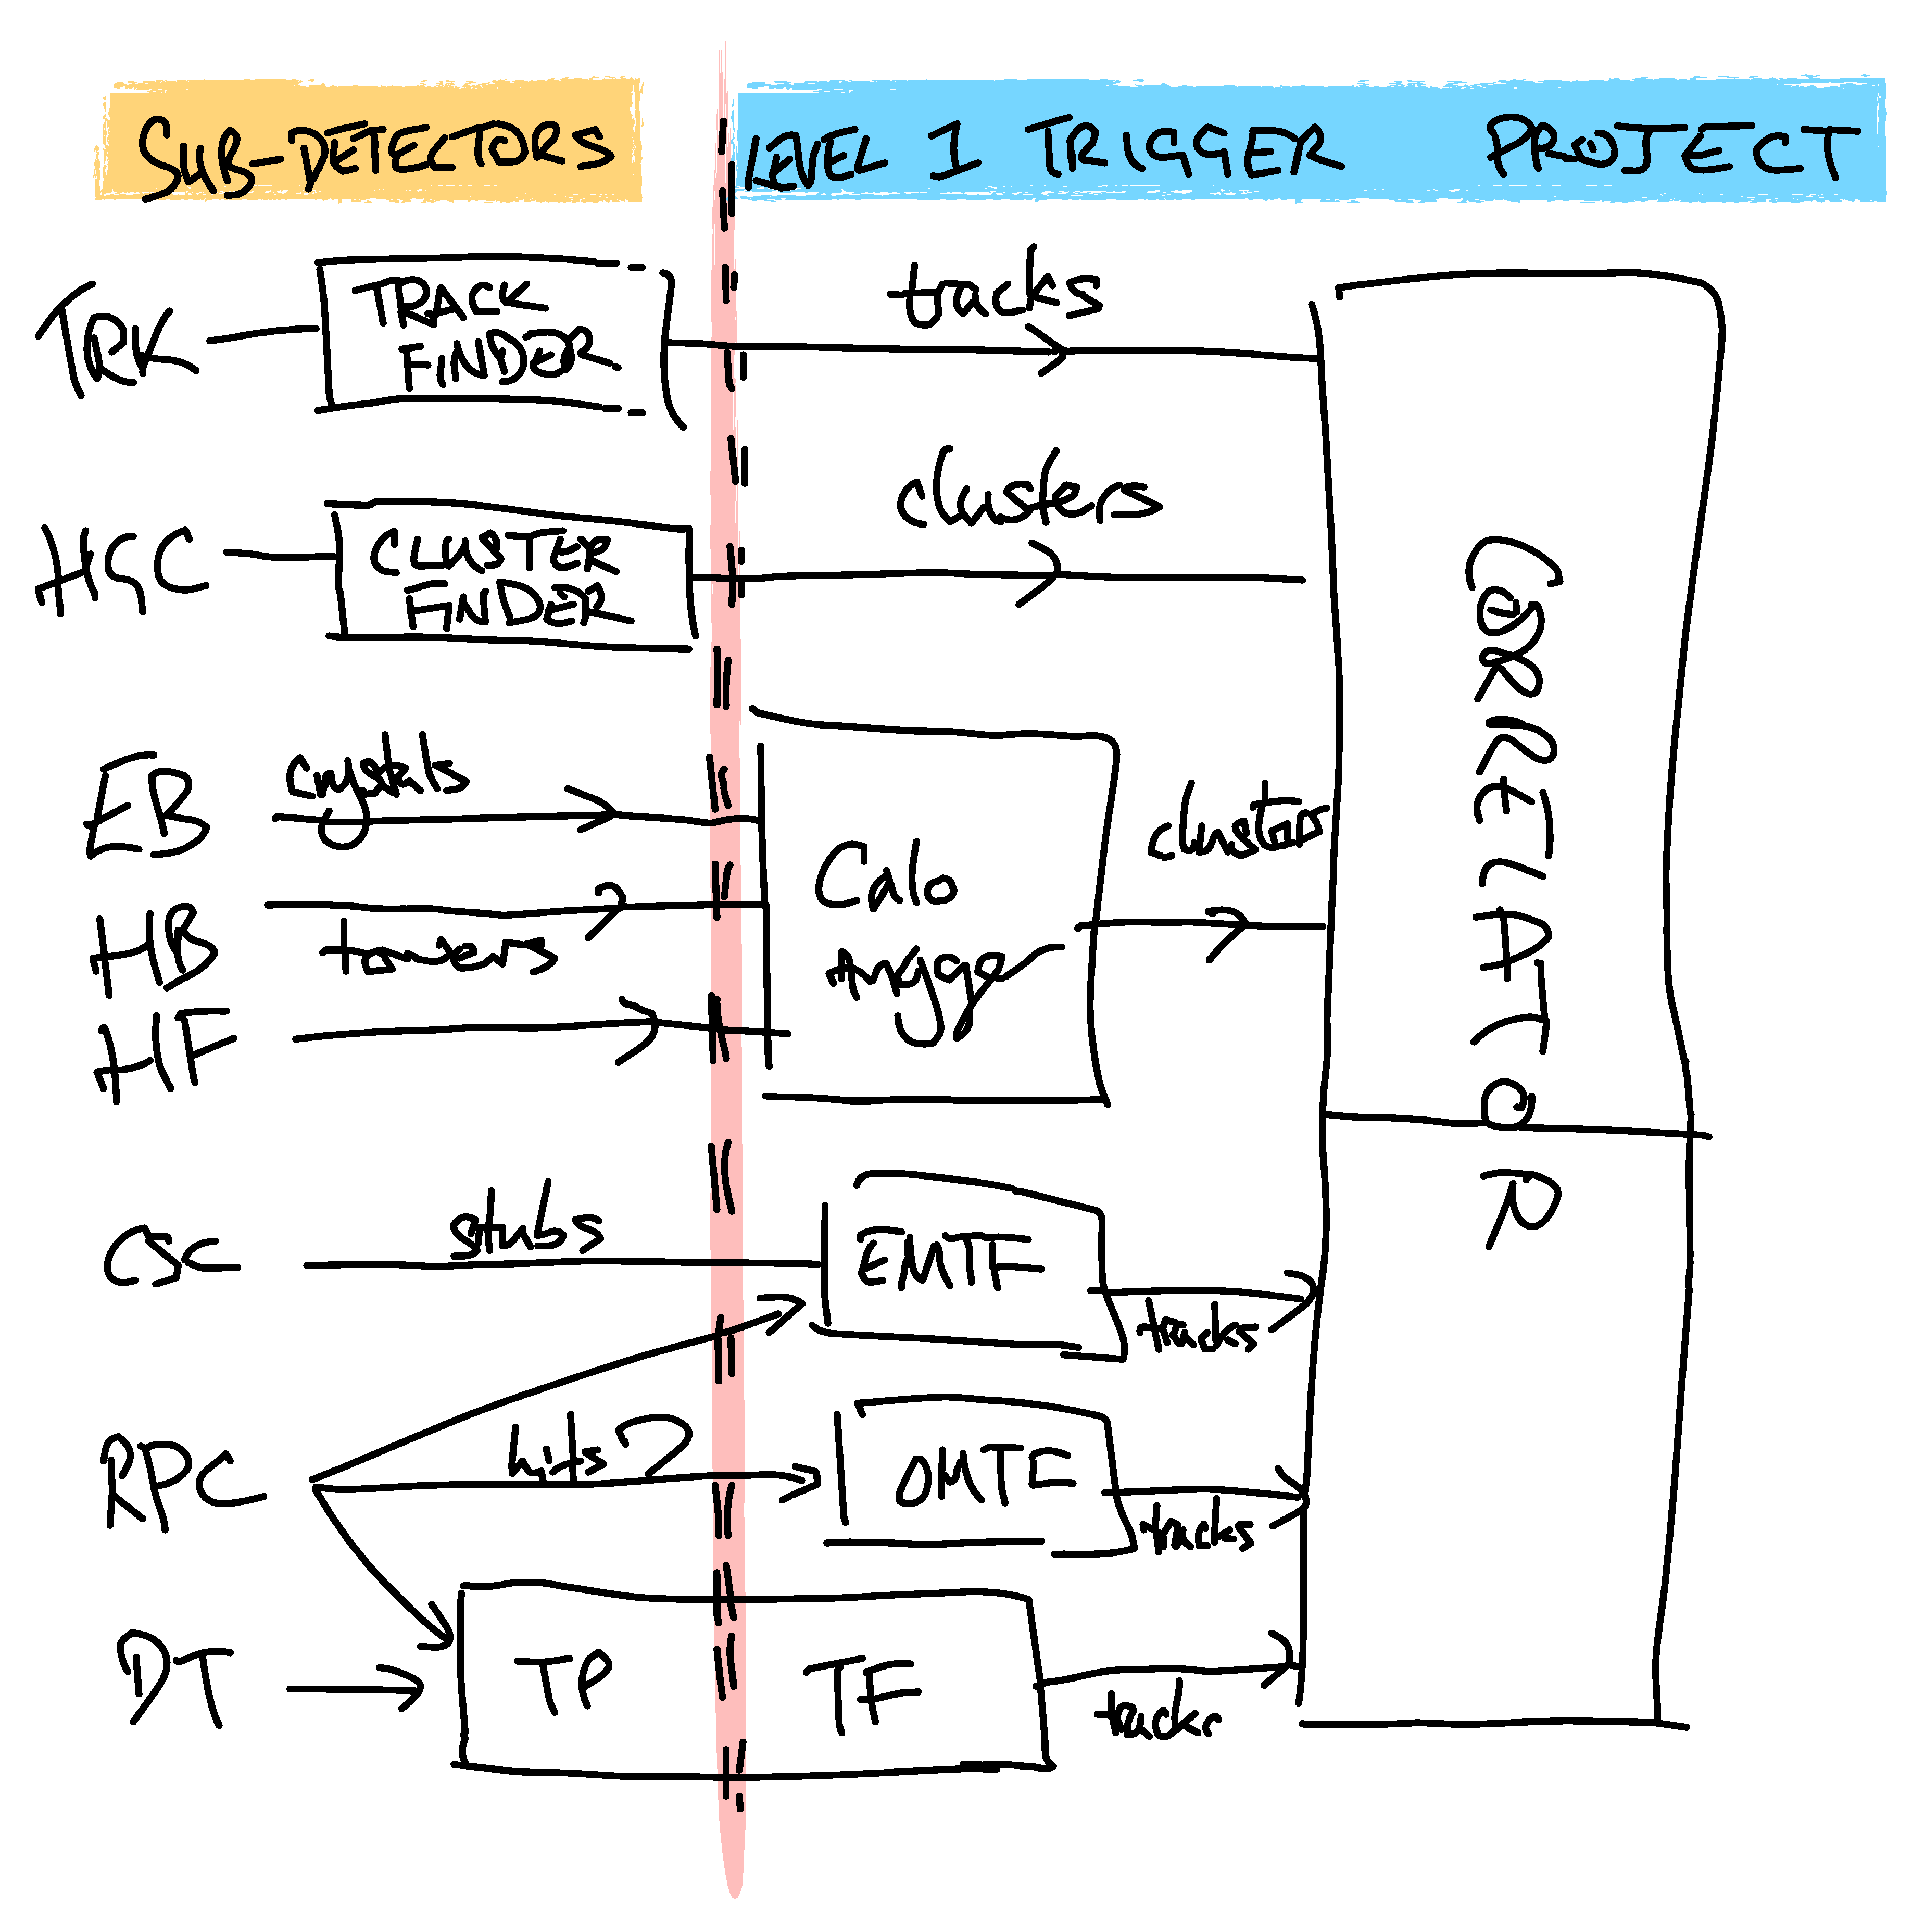
\includegraphics[width=0.6\textwidth] {figures/system.pdf}
\caption{
Overview of the L1 trigger system, courtesy J. Brooke.
\label{fig:overview}
}
\end{figure}

With the addition of the tracking information to the L1 trigger system for the HL-LHC, we can now further expand the capabilities of the system.
Using our experience from offline reconstruction, the particle flow reconstruction algorithm has been successfully demonstrated at CMS.
In this algortihm, detector signals from the tracker, calorimeters and muons are combined and translated into particle candidates such as muons, electrons, charged hadrons, neutral hadrons and photons.
The particle flow algorithm has shown improved physics object resolution and efficiency over more traditional reconstruction techniques. 
In high pileup scenarios, the pileup per particle identification (PUPPI) algorithm, which operates with particle flow candidates as inputs, has been demonstrated to greatly mitigate the physics performance degradation from pileup.  
PUPPI uses vertexing information from the tracks and a QCD-based ansatz to define a weight
of how likely each particle candidates is from pileup.  
The goal of our studies is to implement the principles which make the offline PF and PUPPI algorithms successful 
in the L1 trigger.  

The note is organized as follows.
In Sec.~\ref{sec:algo}, we present the core algorithm in the trigger from hereto on denoted as L1PFP.
In Sec.~\ref{sec:phys}, we then study the physics performance of the algorithm. 
Section~\ref{sec:degradedpf} is devoted to understanding the performance the offline PF and PUPPI algorithms with degraded inputs similar to the trigger.  This is important to benchmark our performance expectations.  
Finally, Sec.~\ref{sec:fw} is devoted to the description of the algorithm and how it is performing in firmware and hardware.  




